\documentclass[a4paper]{article}

\usepackage[portuguese]{babel}
\usepackage[utf8]{inputenc}
\usepackage{amsmath}
\usepackage{graphicx}
\usepackage[colorinlistoftodos]{todonotes}
\usepackage{tabularx,ragged2e,booktabs,caption}


\usepackage{float}
% definitions
\definecolor{blue}{RGB}{159, 192, 176}
\definecolor{green}{RGB}{160, 227, 127}
\definecolor{orange}{RGB}{243, 188, 125}
\definecolor{red}{RGB}{253, 123, 84}
\definecolor{nephritis}{RGB}{39, 174, 96}
\definecolor{emerald}{RGB}{46, 204, 113}
\definecolor{turquoise}{RGB}{39, 174, 96}
\definecolor{green-sea}{RGB}{22, 160, 133}

% Tikzstyles for Computation Graphs

% nodes
\tikzstyle{noop} = [circle, draw=none, fill=red, minimum size = 10pt]
\tikzstyle{op} = [circle, draw=red, line width=1.5pt, fill=red!70, text=black, text centered, font=\bf \normalsize, minimum size = 25pt]
\tikzstyle{state} = [circle, draw=blue, line width=1.5pt, fill=blue!70, text=black, text centered, font=\bf \normalsize, minimum size = 25pt]
% \tikzstyle{gradient} = [circle, draw=green, line width=1.5pt, fill=green!60, text=black, text centered, font=\bf \normalsize, minimum size = 25pt]
\tikzstyle{gradient} = [circle, draw=nephritis, line width=1.5pt, fill=nephritis!60, text=black, text centered, font=\bf \normalsize, minimum size = 25pt]
\tikzstyle{textonly} = [draw=none, fill=none, text centered, font=\bf \normalsize]

% edges
% \tikzstyle{tedge}  = [draw, thick, >=stealth, ->]
\tikzstyle{tedge}  = [draw, thick, >=latex, ->]

% namedscope
\tikzstyle{namedscope} = [circle, draw=orange, line width=1.5pt, fill=orange!60, align=center, inner sep=0pt]

% \tikzstyle{container} = [draw=none, rectangle, dotted, inner ysep=1.5em]
% \tikzstyle{novertex} = [draw=none, fill=none, text centered]
% \tikzstyle{predicate} = [ellipse, draw, thick, text centered, rounded corners, minimum size=30pt]
% \tikzstyle{aux} = [rectangle, draw, thick, text centered, rounded corners, minimum size=30pt]
% \tikzstyle{ledge}  = [draw, dashed, thick, >=stealth, ->]
% \tikzstyle{pedge}  = [draw, thick, >=stealth, ->]



\title{Relatório Intercement: Dados CAJ 2008-2018}

\author{Thiago Ildeu Albuquerque Lira}

\date{\today}

\begin{document}
\maketitle

\newpage
\tableofcontents

\newpage

\section{Introdução}

Esse trabalho surge de uma colaboração entre a empresa Intercement e o Laboratório de Inteligência Artificial e Métodos Formais do IME-USP. Foram concedidos 10 anos de dados de diversas etapas da produção de cimento de uma fábrica. Esse documento apresenta um estudo com a análise desses dados, desde a sua limpeza até uma criação de modelos preditivos para os mesmos.

Os dados foram primeiramente convertidos para formato \textbf{csv} e então importados para o ambiente Python, usando as bibliotecas pandas, matplotlib, numpy, keras e sklearn.

A finalidade de um modelo estatístico é gerar algum tipo de previsão a partir de uma entrada, dessa maneira estimando alguma distribuição de probabilidade $p$ não conhecida ou descobrindo um conjunto de parâmetros que minimize o erro de predição. Para esse projeto serão considerados dados de entrada os dados provenientes dos arquivos com dados de clínquer, farinha e cimento cru. Será tentado em um primeiro momento a simulação dos dados de Expedição a partir de um desses de cada vez e.g. usar os dados de cimento cru de um lote de cimento para prever os dados de expedição desse mesmo lote.


\section{Limpeza dos Dados}

\subsection{Contagem de dias válidos}

Para treinar algum tipo de modelo preditivo com os dados, é necessário parear dados de entrada e de saída. Para os diversos conjuntos de dados cedidos pela Intercement, os mesmos representam diferentes momentos da produção de cimento. Então ao usarmos algum desses dados como entrada para prever uma saída, devemos adicionar o delay temporal correspondente ao tempo que demora para entrada se tornar saída. Por exemplo, se tentarmos prever os dados de expedição com os dados de farinha, o delay apropriado é de 10 dias. No restante desse documento esse delay sempre foi considerado independente de quais dados estejam sendo usados.

Também devemos notar o fato que a frequência na qual os dados de Clínquer, Farinha e Cimento Cru são anotados é bastante maior que a frequência temporal dos dados de expedição. O que também dificulta o pareamento. Por exemplo, temos dados de Clínquer a cada hora, sendo que os dados de expedição são anotados dia a dia. Portanto, foi necessário unir dados de um mesmo dia (tirando a média das suas entradas) para que fosse possível associar diferentes conjuntos de dados de um para um.
\begin{enumerate}
    \item Os dados de  Clínquer possuem 3528 linhas de dados de 2936 dias distintos
\item Os dados de  Expedição possuem 3650 linhas de dados de 2520 dias distintos
\item Os dados de  Farinha possuem 3530 linhas de dados de 2937 dias distintos
\item Os dados de  Cru possuem 30558 linhas de dados de 30558 dias distintos
\end{enumerate}

\subsection{Dados faltantes}
Embora tenhamos uma quantidade razoável de dias com dados presentes, esses muitas vezes não possuem alguma de suas colunas.
A seguir vemos para todos os dataframes, para cada uma de suas colunas, quantos dias possuem dados faltantes.



\captionof{table}{Dias com dados faltantes para cada parâmetro de Clínquer}
\begin{center}
\begin{tabular}{ c c }
 CaOL       &      596\\
Fe2O3       &    596\\
CaO         &   596\\
SiO2        &  596\\
Al2O3       & 596\\
P2O5        & 596\\
MgO         & 596\\
K2O         & 596\\
Na2O        & 596\\
CLOR        & 2724\\
FLUOR       & 2095\\
MS          & 596\\
MA          & 596\\
FSC         & 596\\
RSA         & 809\\
C3S         & 596\\
C2S         & 596\\
C3A         & 596\\
C4AF        & 596\\
F.liq       & 596\\
25,4 mm     & 2753\\
12,7 mm     & 2752\\
6,35  mm    & 2752\\
3,36 mm     & 2752\\
\textless 3,36 mm    & 2756
\end{tabular}
\end{center}
\newpage
\captionof{table}{Dias com dados faltantes para cada parâmetro de Expedição}
\begin{center}
\begin{tabular}{ c c }
AGP     &  1131\\
IP      &  1131\\
FP      &  1132\\
G75    &  1133\\
G44   &  1153\\
MVOL    &  1656\\
SBL     &  1131\\
RC3     &  1130\\
RC7     &  1130\\
RC28    &  1130\\
RICARB  &  1331\\
PF      &  1136\\
AL2O3   &  1140\\
CAOT    &  1140\\
K2O     &  1140\\
MGO     &  1139\\
SIO2    &  1140\\
FE2O3   &  1140\\
SO3     &  1137\\
NA2O    &  3139\\
P2O5    &  1141\\
EXP     &  2804\\
RC1     &  1861\\
RC91    &  3638\\
CO2     &  3629 
\end{tabular}
\end{center}

\newpage

\captionof{table}{Dias com dados faltantes para cada parâmetro de Farinha}
\begin{center}
\begin{tabular}{ c c }
Fe2O3     &   595\\
CaO       &  595\\
SiO2      &   595\\
Al2O3     &   595\\
SO3       &   595\\
P2O5      &   595\\
MgO       &   595\\
K2O       &   595\\
Na2O      &   931\\
CLOR.     &  1697\\
FLUOR.    &  1588\\
FSC       &   595\\
MS        &   595\\
MA        &   595\\
RSA       &   815\\
P. F AL.  &   593 \\
\end{tabular}
\end{center}

\newpage

\captionof{table}{Dias com dados faltantes para cada parâmetro de Cimento Cru}
\begin{center}
\begin{tabular}{ c c }
Alim. (t/h)       & 131\\
Prod (ton)        & 250\\
Calc. (\%)        & 131\\
Arg. (\%)         & 131\\
Areia (\%)        & 132\\
Corr. (\%)        & 370\\
Caulim (\%)       & 421\\
Cinza (\%)        & 295\\
Alurox (\%)       & 442\\
Fe2O3             & 44\\
CaO               & 44\\
SiO2              & 44\\
Al2O3             & 44\\
SO3               & 44\\
P2O5              & 44\\
MgO              &  44\\
K2O              &  44\\
Na2O             &  48\\
MA               &  44\\
MS               &  44\\
FSC              &  44\\
\#100             & 187\\
\#170             &  44\\
Umid Calc (\%)   &  413\\
Umid Arg (\%)    &  414 \\
Umid Areia (\%) &    391 \\
\end{tabular}
\end{center}




\subsection{Resample dos dados}
Para maior facilidade de manuseio dos dados. Foi necessário realizar um \textbf{resample}. Os dados foram modificados para que entradas realizadas no mesmo dia sejam unificadas. E dias sem dados foram criados como placeholders para facilidade de vizualiação dos dados. A seguir são reproduzidas as contagens de dados após o resample.


\begin{itemize}
\item Clínquer: Temos dados de entrada do dia 22/04/2008 até o dia 18/12/2017
\item Clínquer: De um período de 3528 dias temos 2932 dias preenchidos com dados de entrada
\item Expedição: Temos dados de entrada do dia 02/01/2008 até o dia 29/12/2017
\item Expedição: De um período de 3650 dias temos 2520 dias preenchidos com dados de entrada
\item Farinha: Temos dados de entrada do dia 20/04/2008 até o dia 18/12/2017
\item Farinha: De um período de 3530 dias temos 2937 dias preenchidos com dados de entrada
\item Cru: Temos dados de entrada do dia 21/04/2008 até o dia 09/12/2016
\item Cru: De um período de 3155 dias temos 2675 dias preenchidos com dados de entrada
\end{itemize}


\section{Testes de Sazonalidade}

Diversas publicações recentes estudam a eficácia de modelos de Deep Learning para predição de séries temporais, como consumo de energia elétrica. Os dados estudados nesse documento são séries temporais dado que são indexados pelo tempo, porém, resta analisar características temporais desses dados. No exemplo do consumo de energia elétrica, poderiamos notar que, ao longo de vários anos presentes nos dados, o consumo de energia de uma certa residência aumenta em determinado mês. Isso seria um fator útil que um modelo poderia aprender para a predição futura do consumo dessa residência. Dados que não possuem nenhuma característica temporal (i.e. a ordem não importa) seriam por exemplo provenientes de um estudo do salário recebido por uma amostra da população dados fatores como gênero, escolaridade e idade. No primeiro exemplo temos um caso de \textbf{sazonalidade} nos dados, algo que pode ser analisado em séries temporais com testes de análise espectral e auto-correlação. Para os dados desse problema, iremos testar a sazonalidade dos preditores de dureza do cimento.

\subsection{Análise Espectral}

Uma maneira de testar sazonalidade de dados indexados temporalmente é usar a técnica de Transformada de Fourier, onde podemos estudar quais frequencias dentro de um espectro podem ser usadas para decompor um sinal (i.e. nossos dados). Para essa análise usamos os índices de dureza contidos nos dados de expedição, de 2008 até 2014 e descartamos a parte imaginária da análise já que nossos dados não possuem parte complexa. Seguem os resultados:


\begin{figure}[H]
\centering
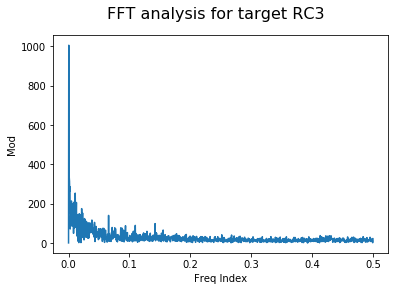
\includegraphics[width=0.9\columnwidth]{images/FFT_RC3.png}
\caption{Análise Espectral para preditor RC3}
\end{figure}

\begin{figure}[H]
\centering
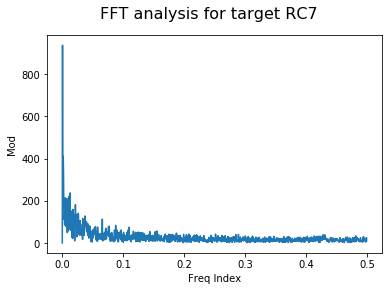
\includegraphics[width=0.9\columnwidth]{images/FFT_RC7.png}
\caption{Análise Espectral para preditor RC7}
\end{figure}

\begin{figure}[H]
\centering
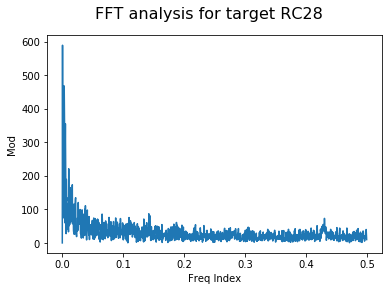
\includegraphics[width=0.9\columnwidth]{images/FFT_RC28.png}
\caption{Análise Espectral para preditor RC28}
\end{figure}


Podemos notar que a "energia" do sinal não possui picos em nenhuma frequência além da frequência zero, que seria a potência média do sinal, ou seja, uma componente que não depende do tempo. Então, afirmamos que esses dados não possuem sazonalidade mensal ou anual. O que significa que a média e a variância desses indicadores não possuem trends e.g. alguma mudança similar todo mês de Janeiro.


\section{Escolha de Modelos}

\subsection{Temporalidade dos Dados}

Pela análise realizada na sessão anterior, podemos concluir que os dados não possuem nenhuma sazonalidade. O problema a ser resolvido para a modelagem desses dados é um problema de aprendizado supervisionado de regressão, e como explicado no início desse documento, devemos fornecer exemplos de entrada e saida para que possivelmente algum modelo aprenda um conjunto de fatores $\theta$ que consigam gerar com alguma acurária novas predições. É importante então sabermos que tipo de informação é útil para darmos como entrada para o modelo. No exemplo da predição de consumo de energia elétrica sabemos que é util para o modelo, além da entrada, ele também receber a \textbf{data} da mesma, pois como foi explicado, esses dados possuem sazonalidade anual. Para os dados de cimento já chegamos a conclusão que a data de uma medida é irrelevante. Porém não descartamos a possibilidade de medidas próximas temporalmente influenciarem uma mesma saída.

Em um problema simples de aprendizado supervisionado gostariamos de aprender uma função $f$ tal que para um par inédito de dados $x^*,y^*$, a nossa função dependa apenas de $x^*$ para que se gere uma predição. Para os dados em questão pode ser que um valor i.e. índice de dureza dependa não só da última entrada, mas de diversas entradas anteriores. 

Ou seja, nossos dados podem ter sido gerados por uma distribuição de probabilidade da forma $p(y | x_{t} ,x_{t -1},x_{t -2},x_{t-3} , \dots, x_{t-T})$, onde uma saida $y$ é condicionada pelas últimas T entradas. Para resolver um problema de aprendizado dessa natureza, devemos usar \textbf{modelos sequenciais}. 

Iremos então experimentar com modelos sequenciais e não-sequencias para testar a acurária de ambos no problema em questão.



\subsection{Inferência Bayesiana}

Será experimentado um modelo sequencial e um modelo não-sequencial que se armem de avanços recentes na área de Machine Learning para que os mesmos possam calcular probabilidades posteriores usando a lei de Bayes. Tais modelos usam uma filosofia diferente para o cálculo de suas predições, estas não sendo mais fruto de maximizar uma verossimilhança ou uma estimativa pontual (achar um conjunto de parâmetros $\theta$ que minimizem alguma métrica de erro). As chamadas Redes Neurais Bayesianas consideram seus parâmetros como distribuições de probabilidade, o que torna cada predição uma ação estocástica, permitindo que sejam calculadas variâncias para cada predição, podendo assim o engenheiro de dados calcular a incerteza do problema.

Uma maneira de implementar uma Rede Neural Bayesiana é usar a técnica Monte Carlo Dropout. Dessa maneira aproximando uma rede neural comum a um processo estocástico sem muitas mudanças no seu código. Usaremos o MC Dropout em uma rede neural clássica (não-sequencial) e em uma RNN (sequencial) para ver como o calculo dessa incerteza auxilia no domínio do problema.

\subsection{Modelo Sequencial}
Com o sucesso de modelos sequenciais no campo do Deep Learning, iremos averiguar se é possível modelar sequencialmente os dados da produção de cimento usando um desses modelos. O modelo selecionado é de uma classe de modelos que se chamam Redes Neurais Recorrentes, ilustrado a seguir:
\\



\scalebox{1}{
\begin{tikzpicture}[auto]

% RNN state cell =============================
\node[state] (h) {$\vect{h}$};
\node[op, below=30pt of h] (x) {$\vect{x}$};
\node[op, above=30pt of h] (yhat) {$\hat{\vect{y}}$};



% edges
\path[tedge] (x) edge node[below right= -4pt] {$\vect{U}$}  (h) ;
\path[tedge] (h) edge [out=-400,in=-320,looseness=8, distance=125pt] node[above right] {$\vect{W}$} (h);
\path[tedge] (h) edge node[below right = -4pt] {$\vect{V}$} (yhat);


\end{tikzpicture}
} % scalebox


Como podemos ver na imagem, a entrada $x$, ao lado do estado interno $W$, são usados para gerar uma predição. Essa por sua vez é comparada com o nosso dado real para que se calcule um erro. O estado $W$ é calculado em cada iteração e usado no cálculo da próxima predição. De modo que esse estado é capaz de transmitir temporalmente ao longo do treinamento informações de dados anteriores.
\\

Essa classe de modelos normalmente é usada para modelagem de linguagem. Buscando estimar uma distribuição de probabilidade $p(w_t | w_{t-1},w_{t-2},w_{t-3} \dots ) $ onde os $w_i$ são palavras subsequentes de um texto. Normalmente um modelo dessa natureza busca resolver um problema de classifição, onde a próxima palavra a ser prevista pelo modelo é uma entre todas as possibilidades de um certo vocabulário. No caso do domínio em questão desejamamos resolver um problema de regressão, onde nosso alvo é um valor numérico. Para treinar um desses modelos, precisamos usar como entrada exemplos subsequentes de dados, onde cada exemplo de entrada tem um exemplo pareado de saída. Basicamente redes neurais recorrentes funcionam recebendo um exemplo de entrada, criando uma representação interna com o mesmo e então gerando uma saída e comparando essa saída com o exemplo de saída real, gerando um erro. Finalmente, esse erro é propagado para alterar seus parâmetros (com o fim de achar um conjunto de parâmetros que gere boas previsões). Podemos vizualizar esse modelo também ao longo do tempo na imagem a seguir:


% RNN STATE CELL ====================================
\newcommand{\rnnSimple}[4]{

% operations
\node[state, minimum size=40pt,#4] (h#3) {$\vect{h}^{#1}$};
\node[op, minimum size=40pt,below=30pt of h#3] (x#3) {$\vect{x}^{#1}$};
\node[op, minimum size=40pt, above=30pt of h#3] (yhat#3) {$\hat{\vect{y}}^{#1}$};

% edges
\path[tedge] (x#3) edge node[below right= -4pt] {$\vect{U}$} (h#3);
\path[tedge] (h#3) edge node[below right = -4pt] {$\vect{V}$} (yhat#3);
}

\begin{figure}[H]
\hspace*{-1.0cm}
\scalebox{0.9}{
\begin{tikzpicture}[auto]

% timestep 1
\rnnSimple{(1)}{(0)}{t1}{}

% % timestep 0
\node[state, minimum size=40pt,left=50pt of ht1] (ht0) {$\vect{h}^{(0)}$};

% % timestep 2
\rnnSimple{(2)}{(1)}{t2}{right=50pt of ht1};


% % timestep 2
\rnnSimple{(3)}{(1)}{t3}{right=50pt of ht2};


% % state transfers
\path[tedge] (ht0) edge node[above right = 2pt] {$\vect{W}$} (ht1);
\path[tedge] (ht1) edge node[above right = 2pt] {$\vect{W}$} (ht2);
\path[tedge] (ht2) edge node[above right = 2pt] {$\vect{W}$} (ht3);

\end{tikzpicture}
}%\scalebox
\end{figure}



Essa imagem mostra exatamente o mesmo modelo da imagem anterior, porém, agora visualizamos o modelo a cada iteração temporal. O estado W é usado como entrada juntamente com o proximo $x_i$ para uma nova iteração.

\bigskip

Como já explicado anteriormente, nossos dados de entrada e saída não estão necessariamente pareados perfeitamente dia a dia. Portanto, foi necessário achar intervalos de tempo nos dados onde existe esse pareamento. Isso reduz drasticamente quais períodos representados nos dados realmente podem ser usados para treinar um desses modelos.



\subsection{Modelo não-sequencial}



Iremos comparar os resultados da RNN com diveros modelos estáticos, ou seja, que não tem a capacidade de modelar nenhuma característica temporal dos nossos dados. Assim como no caso das RNNs, esses modelos funcionam pelo pareamento de entradas e saídas. Porém, nesses modelos, a saída depende unicamente de sua entrada correspondente, o modelo não transmite um estado interno ao longo do treinamento.



\subsubsection{Redes Neurais}




É interessante notar que uma rede neural é equivalente a realizar uma regressão logística por neurônio. Sendo que uma rede neural com apenas um neurônio é uma regressão logística dos dados. A seguir está reproduzida uma rede neural simples com uma camada oculta e dois neurônios de saída.




\begin{figure}[H]
\centering

\scalebox{0.7}{
\begin{tikzpicture}[auto]

% operations =============================

% input layer
\node[op] (x5) {$x_5$};
\node[op, above=2.5pt of x5] (x4) {$Fe_2O_3$};
\node[op, above=2.5pt of x4] (x3) {$CaO$};
\node[op, above=2.5pt of x3] (x2) {$SiO_2$};
\node[op, above=2.5pt of x2] (x1) {$Al_2O_3$};
\node[op, below=2.5pt of x5] (x6) {$SO_3$};
\node[op, below=2.5pt of x6] (x7) {$P_2O_5$};
\node[op, below=2.5pt of x7] (x8) {$MgO$};
\node[op, below=2.5pt of x8] (x9) {$Na_2O$};
\node[op, below=2.5pt of x9] (x10) {$K_2O$};

% hidden layer
\node[op,  right=130pt of x5] (v2) {$v_2$};
\node[op, below=2.5pt of v2] (v3) {$v_3$};
\node[op, below=2.5pt of v3] (v4) {$v_4$};
\node[op, above=2.5pt of v2] (v1) {$v_1$};

\node[op,  right=40pt of v2] (h2) {$h_2$};
\node[op, below=2.5pt of h2] (h3) {$h_3$};
\node[op, below=2.5pt of h3] (h4) {$h_4$};
\node[op, above=2.5pt of h2] (h1) {$h_1$};


% output layer
\node[op,  right=60pt of h2] (z1) {$RC3$};
\node[op,  right=60pt of h3] (z2) {$RC7$};

%\node[op,  right=50pt of z1] (y1) {$\hat{y}_1$};
%\node[op,  right=50pt of z2] (y2) {$\hat{y}_2$};


% edges input layer to hidden
\path[tedge] (x1) -- (v1);
\path[tedge] (x1) -- (v2);
\path[tedge] (x1) -- (v3);
\path[tedge] (x1) -- (v4);

\path[tedge] (x2) -- (v1);
\path[tedge] (x2) -- (v2);
\path[tedge] (x2) -- (v3);
\path[tedge] (x2) -- (v4);

\path[tedge] (x3) -- (v1);
\path[tedge] (x3) -- (v2);
\path[tedge] (x3) -- (v3);
\path[tedge] (x3) -- (v4);

\path[tedge] (x4) -- (v1);
\path[tedge] (x4) -- (v2);
\path[tedge] (x4) -- (v3);
\path[tedge] (x4) -- (v4);

\path[tedge] (x5) -- (v1);
\path[tedge] (x5) -- (v2);
\path[tedge] (x5) -- (v3);
\path[tedge] (x5) -- (v4);

\path[tedge] (x6) -- (v1);
\path[tedge] (x6) -- (v2);
\path[tedge] (x6) -- (v3);
\path[tedge] (x6) -- (v4);

\path[tedge] (x7) -- (v1);
\path[tedge] (x7) -- (v2);
\path[tedge] (x7) -- (v3);
\path[tedge] (x7) -- (v4);

\path[tedge] (x8) -- (v1);
\path[tedge] (x8) -- (v2);
\path[tedge] (x8) -- (v3);
\path[tedge] (x8) -- (v4);

\path[tedge] (x9) -- (v1);
\path[tedge] (x9) -- (v2);
\path[tedge] (x9) -- (v3);
\path[tedge] (x9) -- (v4);

\path[tedge] (x10) -- (v1);
\path[tedge] (x10) -- (v2);
\path[tedge] (x10) -- (v3);
\path[tedge] (x10) -- (v4);

% edges hidden to hidden
\path[tedge] (v1) edge node[above=1pt] {{\Large$\sigma$}}  (h1) ;
\path[tedge] (v2) edge node[above=1pt] {{\Large$\sigma$}}  (h2) ;
\path[tedge] (v3) edge node[above=1pt] {{\Large$\sigma$}}  (h3) ;
\path[tedge] (v4) edge node[above=1pt] {{\Large$\sigma$}}  (h4) ;

% edges hidden to output
\path[tedge] (h1) -- (z1);
\path[tedge] (h1) -- (z2);

\path[tedge] (h2) -- (z1);
\path[tedge] (h2) -- (z2);

\path[tedge] (h3) -- (z1);
\path[tedge] (h3) -- (z2);

\path[tedge] (h4) -- (z1);
\path[tedge] (h4) -- (z2);

% edges output to output
%\path[tedge] (z1) edge node[above=1pt] {{\Large softmax}}  (y1) ;
%\path[tedge] (z2) edge node[above=1pt] {{\Large softmax}}  (y2) ;




\end{tikzpicture}
} % scalebox
\end{figure}



Na imagem mostramos como seria uma rede que usa como parâmetros alguns dos dados de Farinha para modelar os índices RC3 e RC7 dos dados de expedição.

\bigskip
\subsubsection{Regressão Linear}
Os modelos são também comparados com uma regressão linear. Que usa estimação por mínimos quadrados para calcular um peso para cada parâmetro de entrada. De modo que a soma ponderada por esses pesos possa aproximar nosso alvo.


\subsubsection{Random Forest}

Random Forests são um método de \textbf{Ensemble Learning} para classificação ou regressão. \textbf{Ensemble Learning} são uma técnica no qual diversos modelos "fracos" são usados em conjunto com algum sistema de votação para que a a acurária do sistema em conjunto se torne melhor que a de qualquer um dos modelos sozinho. Seguindo essa ideia, Random Forests são conjuntos de diveras árvores de decisão simples unidas por um meta-algoritmo de votação para que se produza uma predição muito mais eficaz.


\section{Resultados}


Todos os testes foram feitos com normalização min-max dos dados, para que se evite comportamentos estranhos por parte das redes neurais. \\

\bigskip

Como teste da acurácia dos modelos foi usada a métrica R-quadrado. Sejam $\hat{y}$ e $y$ nossa previsão dada pelo modelo e o seu valor real, a acurácia do modelo é dada por:\\

\bigskip

\centering
$R_2 = 1 - \frac{SS_{res}}{SS_{tot}}$\\

$SS_{tot} = \sum (y - \hat{y})^2$

$SS_{res} = \sum (y - \bar{y})^2$

$  \bar{y} = \frac{1}{n} \sum y$
\bigskip

\justify
Para essa métrica, o modelo pode performar arbitrariamente mal, com esse valor podendo se tornar arbitrariamente negativo. Porém, seu valor máximo é 1, indicando um modelo ideal.\\

\bigskip
\subsection{Primeiro Ensaio}
A seguir são reproduzidos gráficos de um experimento realizado com o fim de comparar nossos modelos. Usamos os dados de Farinha para prever os índices RC3, RC7 e RC28. Foi preferido treinar um modelo de cada tipo para cada um dos índices, por simplicidade. Ou seja, são usados parâmetros dos dados de entrada com o fim de prever um único parâmetro de saída. 
\\
\\
Para o treinamento e teste de cada modelo, separamos os dados em duas partes. Nesse experimento os dados de farinha e expedição de 2008 a 2016 foram usados como dados de treinamento e 30\% desses foram aleatóriamente selecionados para servirem de dados de teste, chamado no jargão técnico como \textit{test set}. Finalmente, os dados de 2017 e 2018 foram usados como um segundo conjunto de dados de treinamento, estes em um período completamente inédito para os modelos treinados, esse segundo conjunto chamado por sua vez usualmente de \textit{dev set}. Os gráficos a seguir mostram em azul os dados reais de 2017 em diante, bem como as previsões feitas por cada modelo em laranja. As métricas R-quadrado para cada conjunto de dados de teste também são mostradas no canto inferior direito.



\begin{figure}[H]
\centering
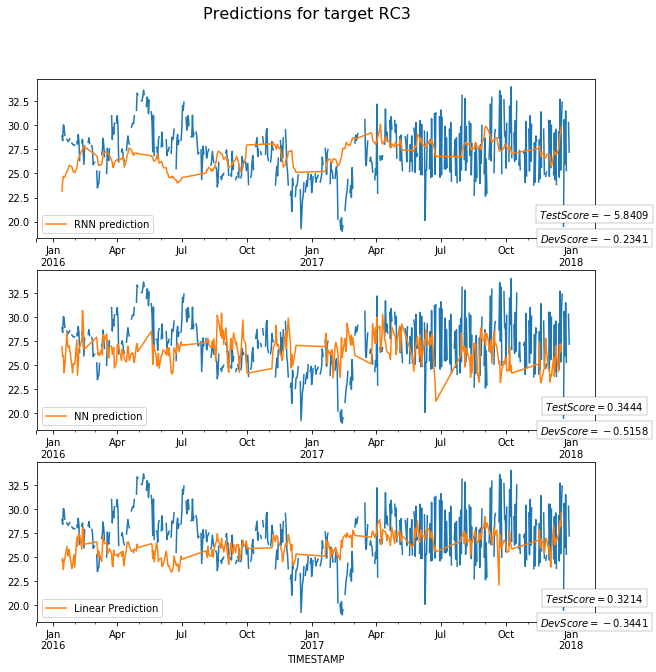
\includegraphics[width=0.9\columnwidth]{images/RC3.png}
\caption{Comparação dos 3 modelos na tarefa de regressão do índice RC3}
\end{figure}

\begin{figure}[H]
\centering
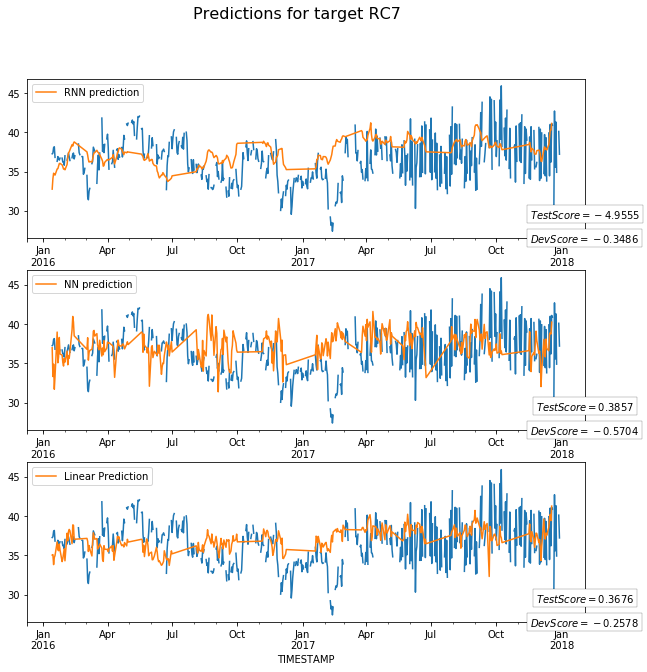
\includegraphics[width=0.9\columnwidth]{images/RC7.png}
\caption{Comparação dos 3 modelos na tarefa de regressão do índice RC7}
\end{figure}

\begin{figure}[H]
\centering
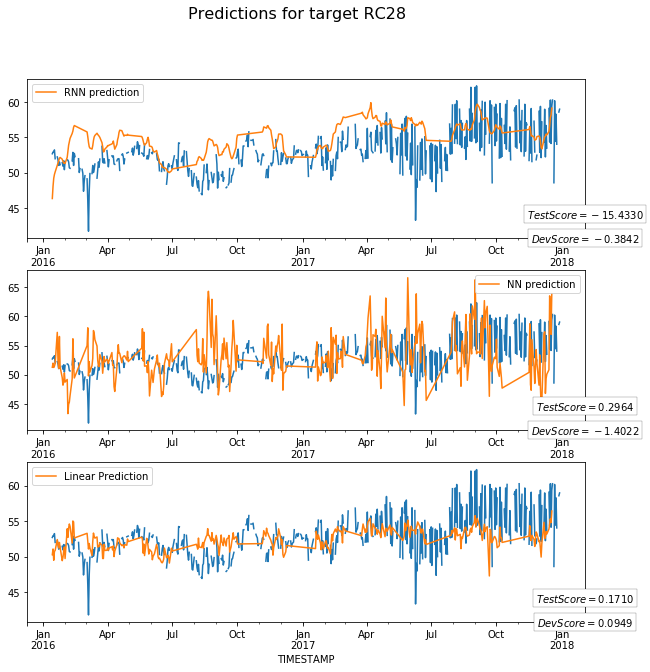
\includegraphics[width=0.9\columnwidth]{images/RC28.png}
\caption{Comparação dos 3 modelos na tarefa de regressão do índice RC28}
\end{figure}


\subsection{Segundo Ensaio}

Estudando os dados vemos que ouve um aumento repentino dos índices de dureza a partir de 2016, e um ruído sensivelmente mais presente e com uma variância maior. Várias tentativas foram feitas com diversos parâmetros de entrada e nenhum conjunto destes ajuda a prever essa mudança brusca nos dados. Portanto devemos concluir que ela é dada por fatores não presentes nos dados concedidos. O primeiro ensaio foi realizado com os dados de treinamento sendo de 2008 a 2015, com o restante sendo nossos dados de validação. Uma performance melhor possivelmente seria atingida se usarmos dados antes de 2016 para treinamento e validação.
\\
\\


Segue um plot da nova divisão dos dados entre treino/teste e validação para os índices que estamos tentando modelar:

\begin{figure}[H]
\centering
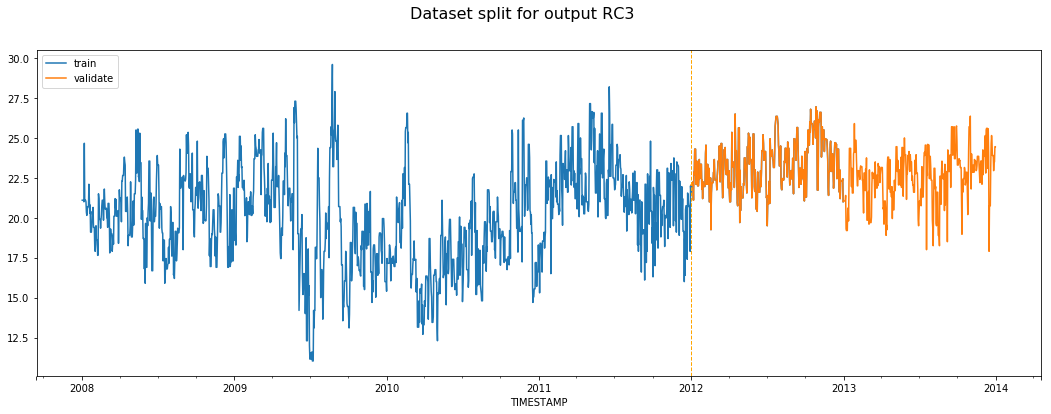
\includegraphics[width=0.9\columnwidth]{images/dataset_splitRC3.png}
\caption{Divisão do dataset para a saída RC3}
\end{figure}

\begin{figure}[H]
\centering
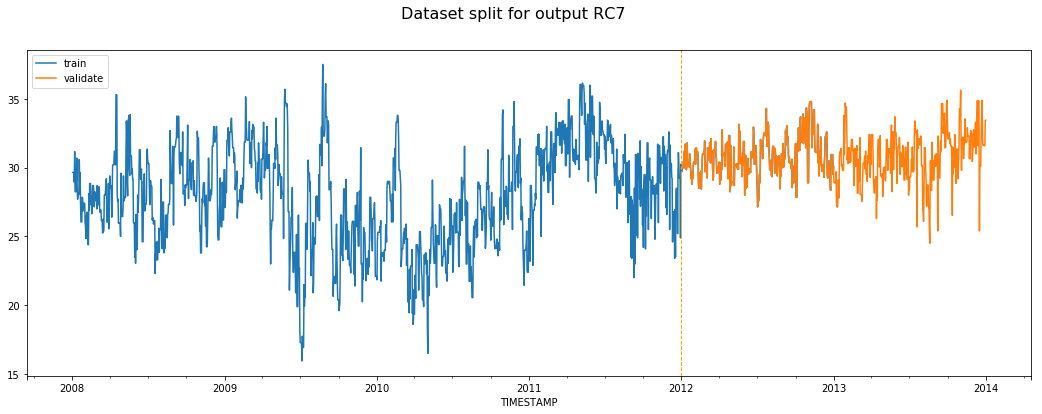
\includegraphics[width=0.9\columnwidth]{images/dataset_splitRC7.png}
\caption{Divisão do dataset para a saída RC7}
\end{figure}

\begin{figure}[H]
\centering
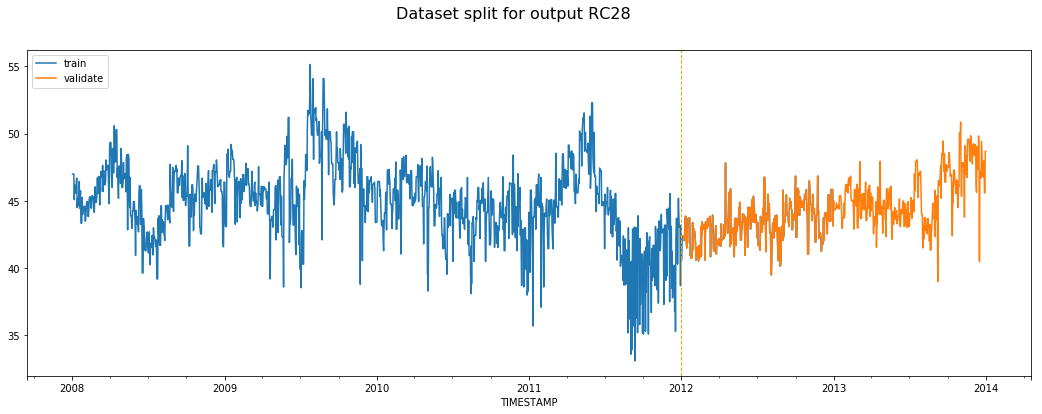
\includegraphics[width=0.9\columnwidth]{images/dataset_splitRC28.png}
\caption{Divisão do dataset para a saída RC28}
\end{figure}

\\
\\

Finalmente, seguem plots dos novos resultados, esses sendo reproduzidos apenas para o período inédito para os modelos, ou seja, o \textbf{dev set} de 2012 até 2014:


\bigskip
Primeiro, os modelos considerando os dados como não-sequenciais:

\begin{figure}[H]
\centering
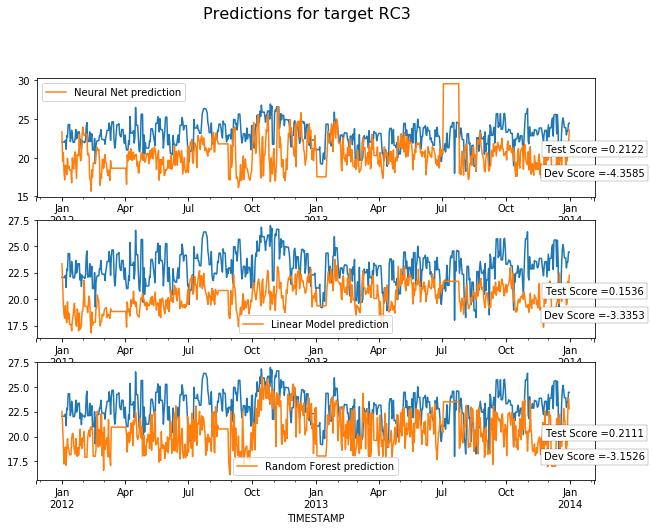
\includegraphics[width=0.9\columnwidth]{images/farinha_2008-2012-2014RC3.png}
\caption{Comparação dos 3 modelos não-sequenciais na tarefa de regressão do índice RC3}
\end{figure}

\begin{figure}[H]
\centering
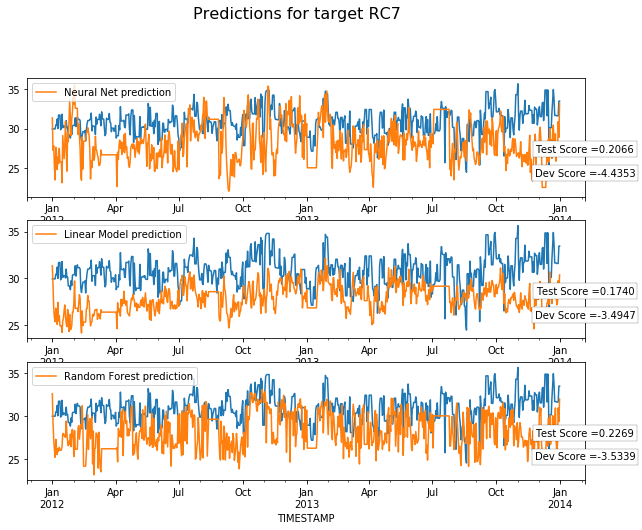
\includegraphics[width=0.9\columnwidth]{images/farinha_2008-2012-2014RC7.png}
\caption{Comparação dos 3 modelos não-sequenciais na tarefa de regressão do índice RC7}
\end{figure}

\begin{figure}[H]
\centering
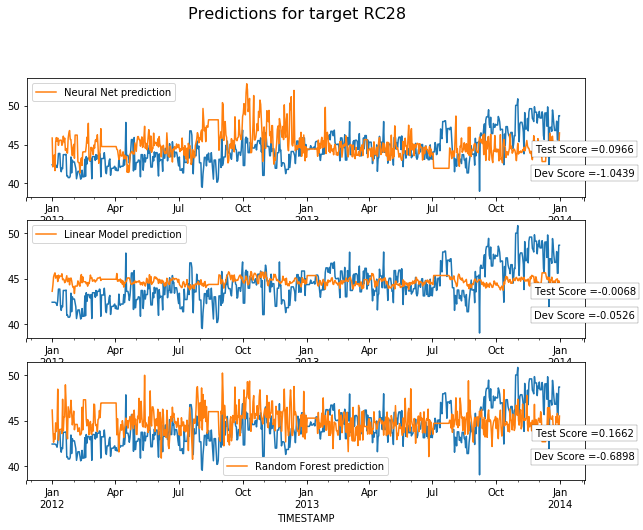
\includegraphics[width=0.9\columnwidth]{images/farinha_2008-2012-2014RC28.png}
\caption{Comparação dos 3 modelos não-sequenciais na tarefa de regressão do índice RC28}
\end{figure}

\\

Agora, a performance da Rede Neural usando a técnica de Monte Carlo Dropout para inferência Bayesiana e cálculo de incerteza:


\begin{figure}[H]
\centering
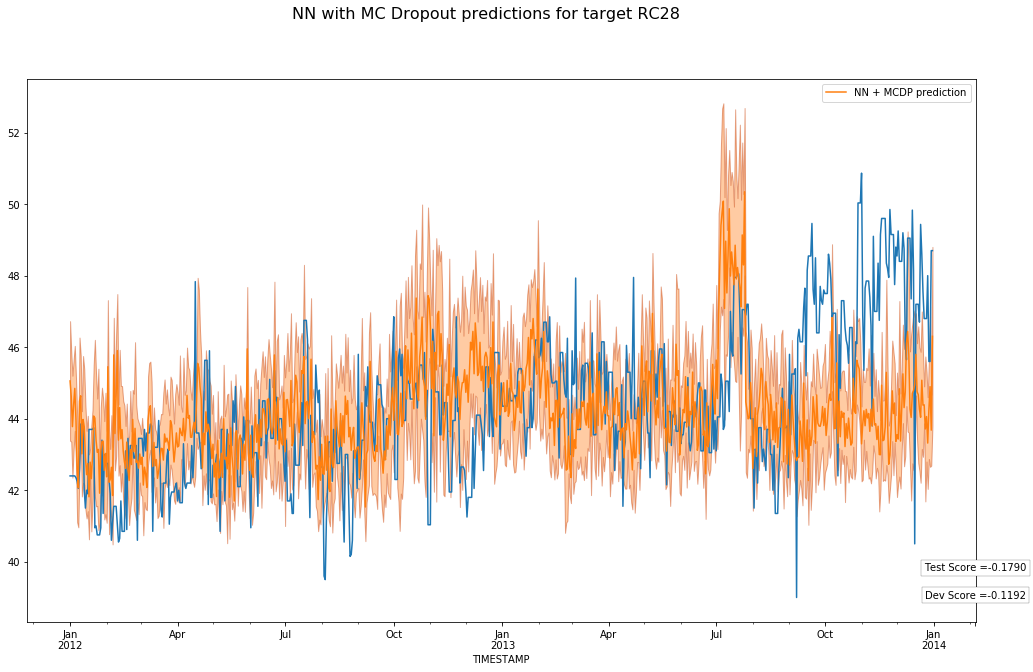
\includegraphics[width=1\columnwidth]{images/NNMCDP_2012-2014RC28.png}
\caption{Performance do modelo Rede Neural + MC Dropout para o índice RC28}
\end{figure}


É interessante notar que o modelo anterior com a sua capacidade de calcular incertezas, realiza uma boa tarefa de "cobrir" os dados reais com a sua incerteza prevista para os pontos de dados previstos.
 \\
 \\

Finalmente, temos o modelo de Rede Neural Recorrente, um modelo sequencial:

\\ 
\\

\begin{figure}[H]
\centering
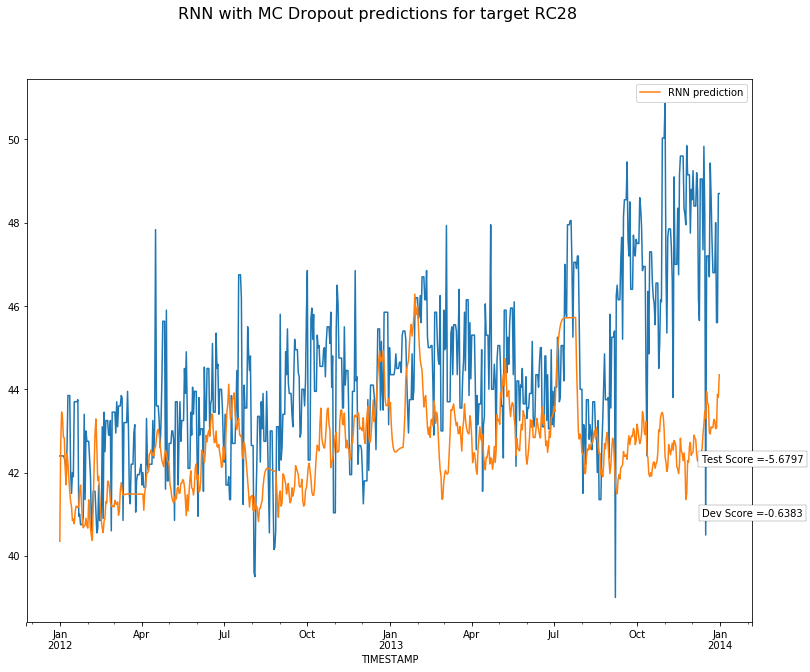
\includegraphics[width=0.9\columnwidth]{images/RNN_2012-2014RC28.png}
\caption{Performance do modelo RNN para o índice RC28}
\end{figure}


\bigskip

Dos resultados obtidos podemos perceber que a acurácia dos modelos aumenta sensivalmente para o índice RC28, isso se dá pelo fato que essa é uma medida na qual naturalmente está envolvido menos ruído e incerteza que as outras duas. Analisando os valores da métrica R2, os melhores modelos atingiram valores próximos de $0$.




\section{Conclusão}

Pelos resultados obtidos, é possível concluir que não houveram ganhos significativos em usarmos modelos sequenciais de Deep Learning na modelagem dos dados. Como uma simples regressão linear consegue em alguns casos até performar melhor que uma rede neural ou uma rede recorrente, podemos afirmar também que a natureza temporal dos dados não é útil na modelagem dos mesmos. A performance de modelos que consideram esses dados não-sequenciais obteve uma performance equivalente ou melhor.

Os dados possuem uma grande quantidade de ruído proveniente de incertezas no instante das medições, o que dificulta o aprendizado seja de qual modelo for usado. E também é claro que ao longo dos 10 anos de dados possuimos mudanças bruscas de valores provenientes de fatores não presentes nos dados. Ou seja, do domínio que queremos aprender temos dados com um ruído alto e variável além de não possuirmos toda a informação do suposto "processo gerador de dados" (a distribuição de probabilidades $p$ que queremos estimar), o que dificulta qualquer modelo estatístico para o qual iremos dar essa tarefa.

Como uma regressão linear consegue resultados comparáveis a modelos diferentes e mais complexos, pode-se afirmar que a distribuição de probabilidade que queremos estimar para os preditores não é muito complexa, mas os fatores mencionados no parágrafo anterior atrapalham uma melhor performance dos modelos usados. Resultados melhores possivelmente podem ser obtidos usando métodos clássicos de Machine Learning como \textbf{feature engineering}, ou seja, aplicar um conhecimento específico do domínio do problema em questão para deixar menos para os modelos decidirem sozinhos. O que é imcompatível com métodos de Deep Learning. 


\end{document}
